\documentclass[aspectratio=43]{beamer}
\usepackage{hyperref, graphicx}
\mode<presentation>

\title{ENPH 253: \textit{El Buscador Del Oro}}
\date{\today}

\author{Reily Blackner \and Tyson Costa\\ \and Todd Darcie \and Oliver Gadsby}
\institute[UBC]{University of British Columbia}

\usecolortheme{whale}
\setbeamercolor{structure}{fg=beamer@blendedblue}
\definecolor{beamer@blendedblue}{rgb}{0.137,0.466,0.741}

\setbeamertemplate{footline}
{
  \begin{beamercolorbox}[colsep=1.5pt]{upper separation line foot}
  \end{beamercolorbox}

  \begin{beamercolorbox}[ht=2.5ex,dp=1.125ex,
    leftskip=.3cm,rightskip=.3cm plus1fil]{author in head/foot}
    \leavevmode{\usebeamerfont{author in head/foot}\insertshortauthor}
    \hfill
    {\usebeamerfont{institute in head/foot}\usebeamercolor[fg]{institute in head/foot}\insertshortinstitute}
  \end{beamercolorbox}

  \begin{beamercolorbox}[ht=2.5ex,dp=1.125ex,
    leftskip=.3cm,rightskip=.3cm plus1fil]{title in head/foot}
    {\usebeamerfont{title in head/foot}\insertshorttitle}
    \hfill
    \insertframenumber/\inserttotalframenumber
  \end{beamercolorbox}
  
  \begin{beamercolorbox}[colsep=1.5pt]{lower separation line foot}
  \end{beamercolorbox}
}

\begin{document}


  \begin{frame}
    \titlepage
  \end{frame} 
  

  \begin{frame}{Introduction}
    \begin{columns}[c]
      \begin{column}[c]{5cm}
        \begin{itemize}
          \item Challenge Objective
          \item Challenge Surface
          \item Overview of Robot
            \begin{itemize}
              \item Chassis and Drive System
              \item Idol Retrieval System (I.R.S.)
              \item Telescoping Return Mechanism (T.R.M.)
              \item Electrical Components
              \item Software Design
            \end{itemize}
        \end{itemize}
      \end{column}
      \begin{column}[c]{5cm}
        
\includegraphics[<options, e.g. width=\textwidth>]{ENPHlogo.png}
      \end{column}
    \end{columns}
  \end{frame} 
  

  \begin{frame}{Challenge Objective}
    \begin{columns}[c]
      \begin{column}[c]{5cm}
        \begin{itemize}
          \item Tape Follow
          \item Collect Artifacts
          \item Detect and Follow IR Beacon
          \item Return to Start with Artifacts and Golden Idol
        \end{itemize}
      \end{column}
      \begin{column}[c]{5cm}
        \begin{figure}[h]
          \centering
          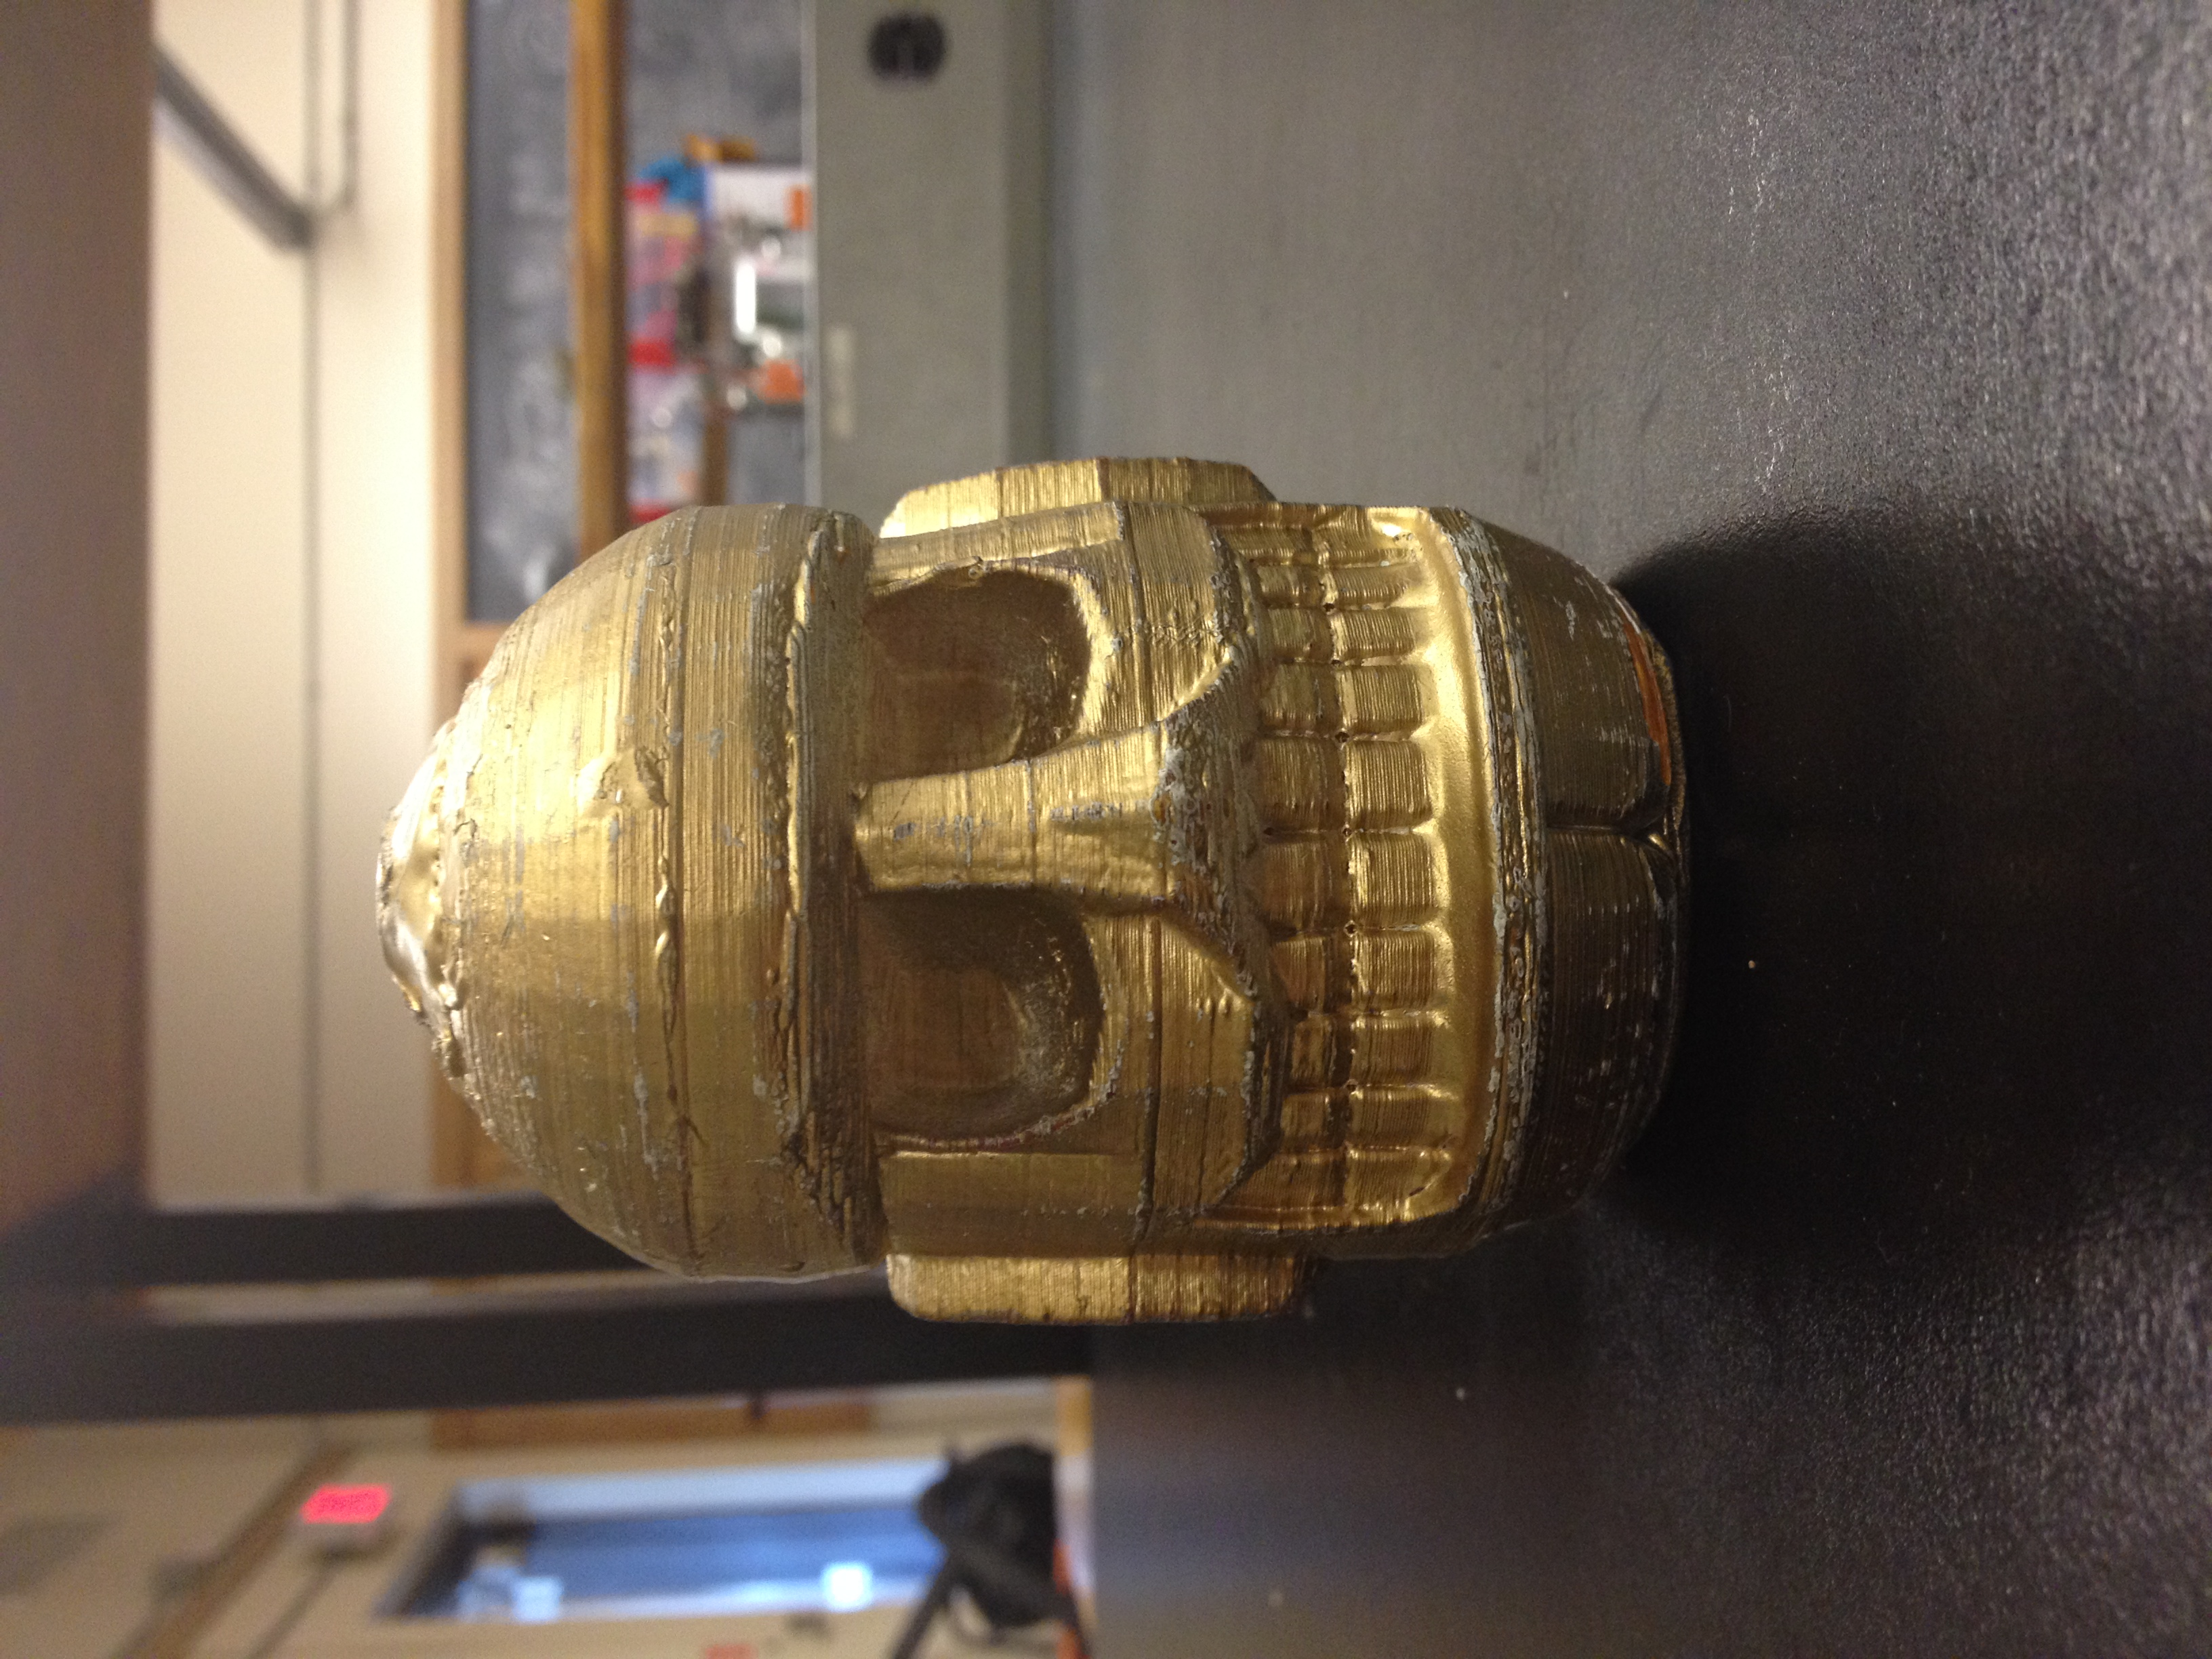
\includegraphics[scale = 0.05, angle=-90]{GoldIdol.jpeg}
          \vspace{7pt}
          \large{Golden Idol}
        \end{figure}
      \end{column}
    \end{columns}
  \end{frame} 
  

  \begin{frame}{Challenge Surface}
    \begin{center}
      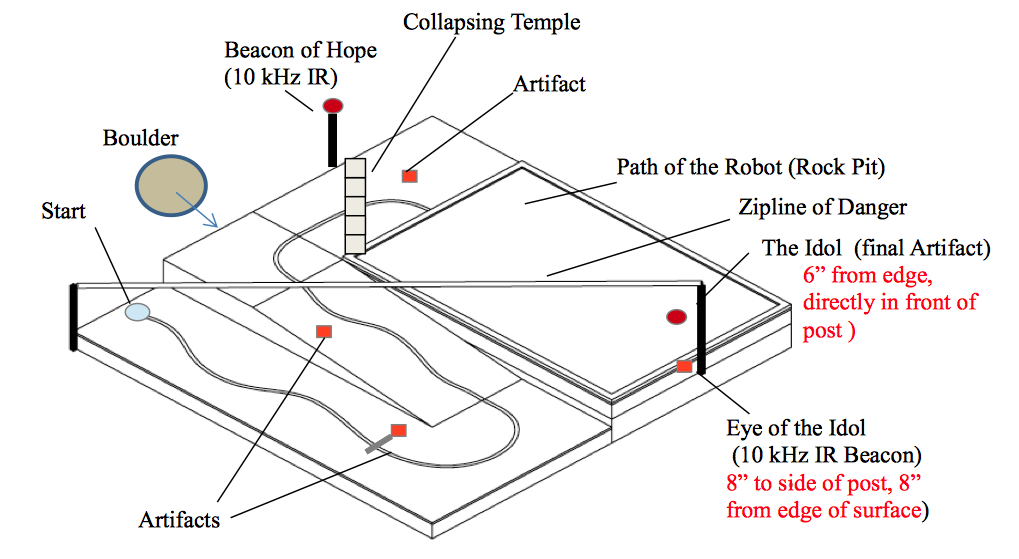
\includegraphics[scale = 0.3]{Course.png}
    \end{center}
  \end{frame} 
  

  \begin{frame}{\textit{El Buscador del Oro}}
    \begin{center}
      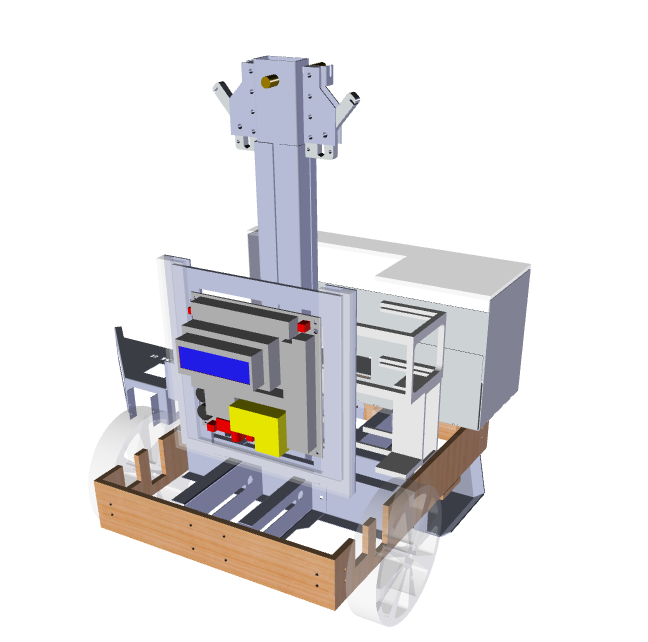
\includegraphics[scale = 0.3]{BuscDelOro.png}
    \end{center}
  \end{frame} 
  

  \begin{frame}{Chassis and Drive System}
    \begin{columns}[c]
      \begin{column}[c]{5cm}
        \begin{itemize}
          \item Gearbox and Motors
          \item Wheels and Sleds
          \item Suspension
        \end{itemize}
      \end{column}
      \begin{column}[c]{5cm}
        \begin{figure}[h]
          \centering
          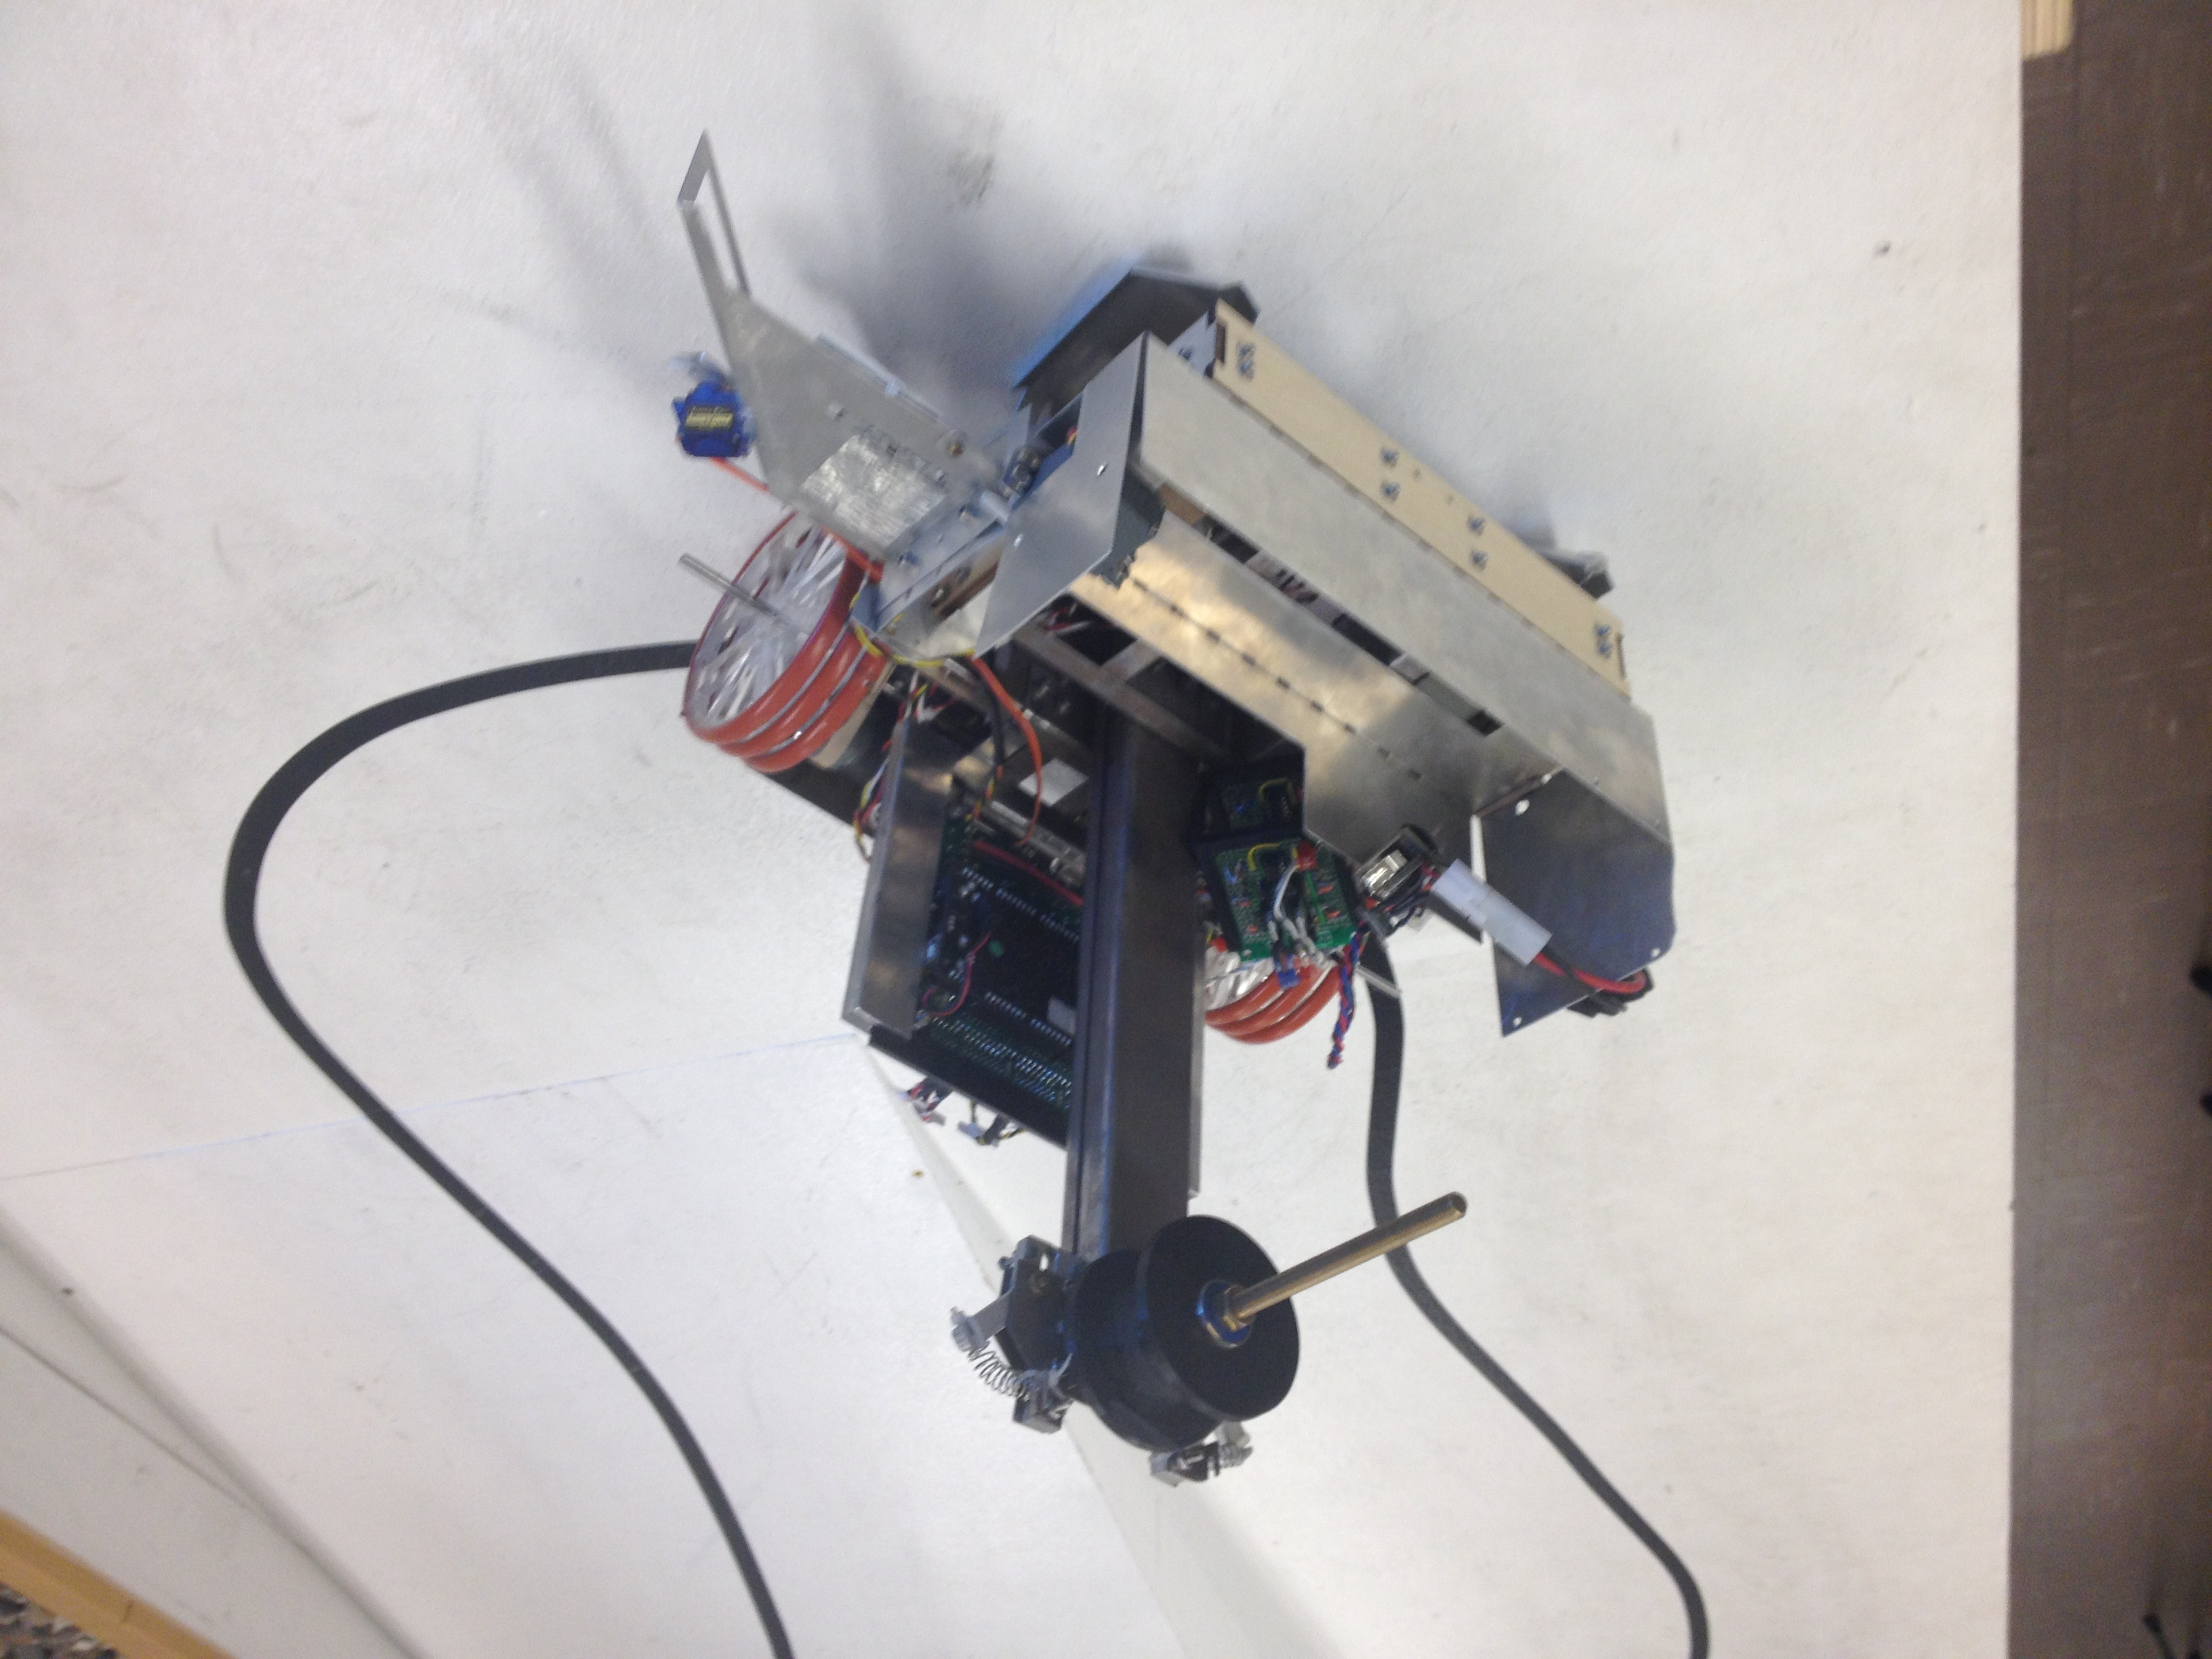
\includegraphics[scale = 0.05, angle=180]{Chassis.JPG}
          \vspace{7pt}
          \large{Chassis}
        \end{figure}
      \end{column}
    \end{columns}
  \end{frame} 
  

  \begin{frame}{Idol Retrieval System (I.R.S.)}
    \begin{columns}[c]
      \begin{column}[c]{5cm}
        \begin{itemize}
          \item Collector Arm
          \item Sweeper Arm
          \item Basket and Conveyor Belt
        \end{itemize}
      \end{column}
      \begin{column}[c]{5cm}
        \begin{figure}[h]
          \centering
          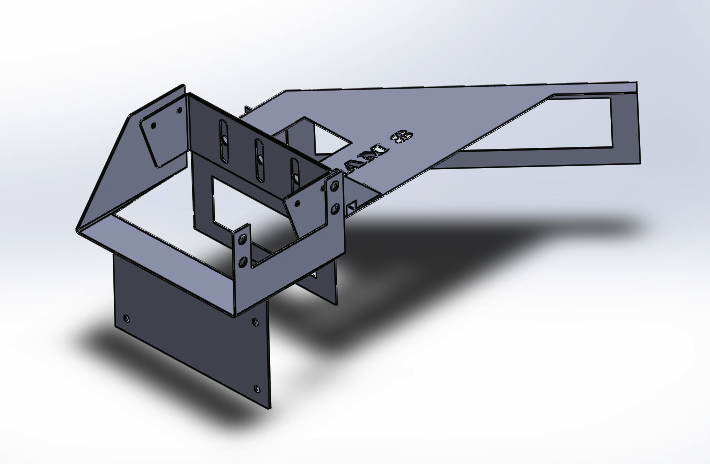
\includegraphics[scale = 0.225]{IRS.png}
          \vspace{7pt}
          \large{IRS}
        \end{figure}
      \end{column}
    \end{columns}
  \end{frame} 
  

  \begin{frame}{Telescoping Return Mechanism (T.R.M.)}
    \begin{columns}[c]
      \begin{column}[c]{5cm}
        \begin{itemize}
          \item Telescoping Arms
          \item Winch
          \item Rubber Bands
          \item Release System
          \item Zipline Wheel
        \end{itemize}
      \end{column}
      \begin{column}[c]{5cm}
        \begin{figure}[h]
          \centering
          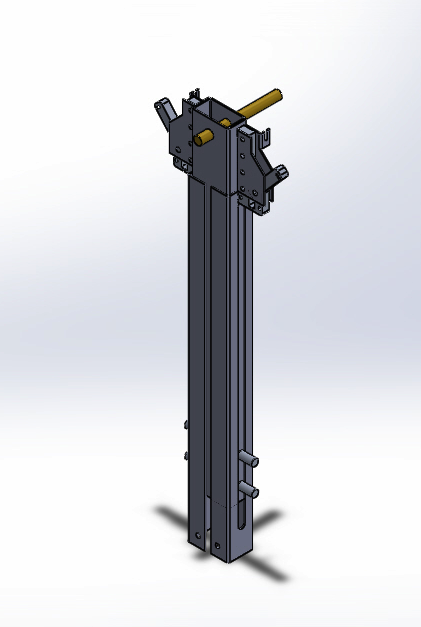
\includegraphics[scale = 0.275]{TRM.png}
          \vspace{7pt}
          \large{TRM}
        \end{figure}
      \end{column}
    \end{columns}
  \end{frame} 


  \begin{frame}{Electrical Components}
    \begin{columns}[c]
      \begin{column}[c]{5cm}
        \begin{itemize}
          \item H-Bridge Circuit
          \item Infrared Detection Circuit
          \item Reflective Object Sensors (QRDs)
        \end{itemize}
      \end{column}
      \begin{column}[c]{5cm}
        \begin{figure}[h]
          \centering
          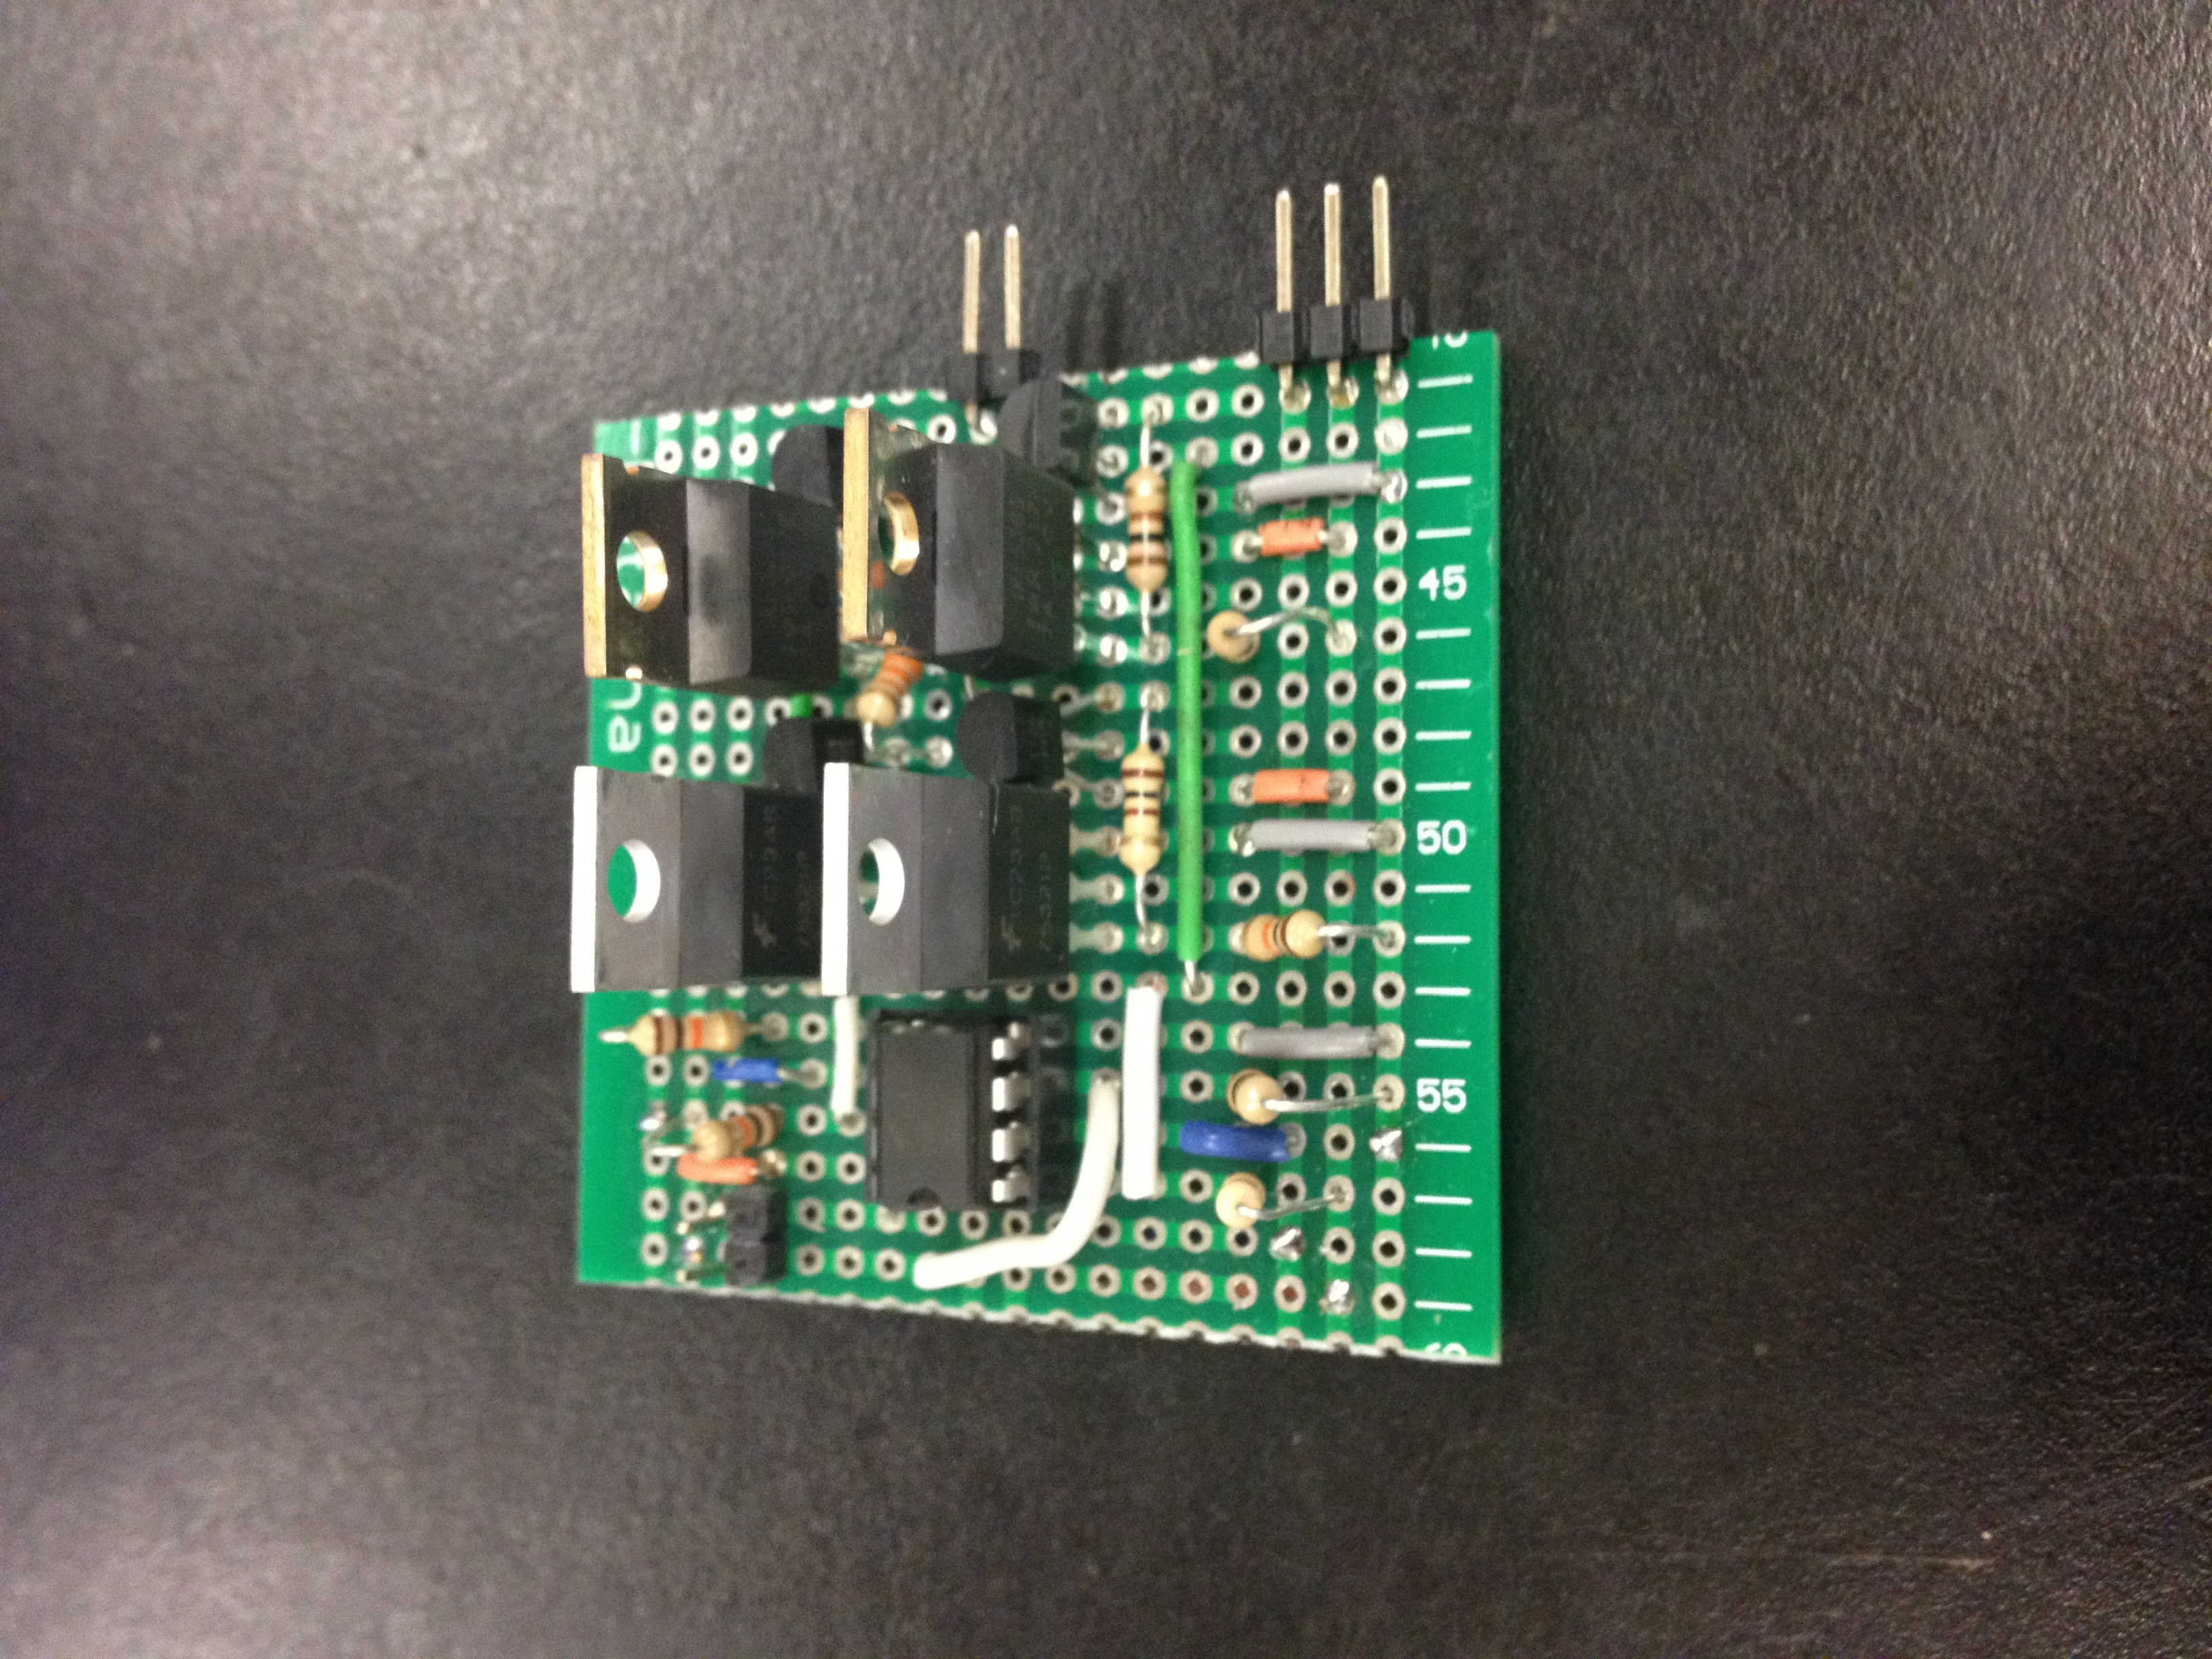
\includegraphics[scale=0.05, angle=-90]{HBridge.jpeg}
          \vspace{7pt}
          \large{H-Bridge}
        \end{figure}
      \end{column}
    \end{columns}
  \end{frame} 
  

  \begin{frame}{Software Design}
    \begin{columns}[c]
      \begin{column}[c]{5cm}
        \begin{itemize}
          \item Test Based Programming
          \item Saving Data
          \item TINAH Menu System
        \end{itemize}
      \end{column}
      \begin{column}[c]{5cm}
        \begin{figure}[h]
          \centering
          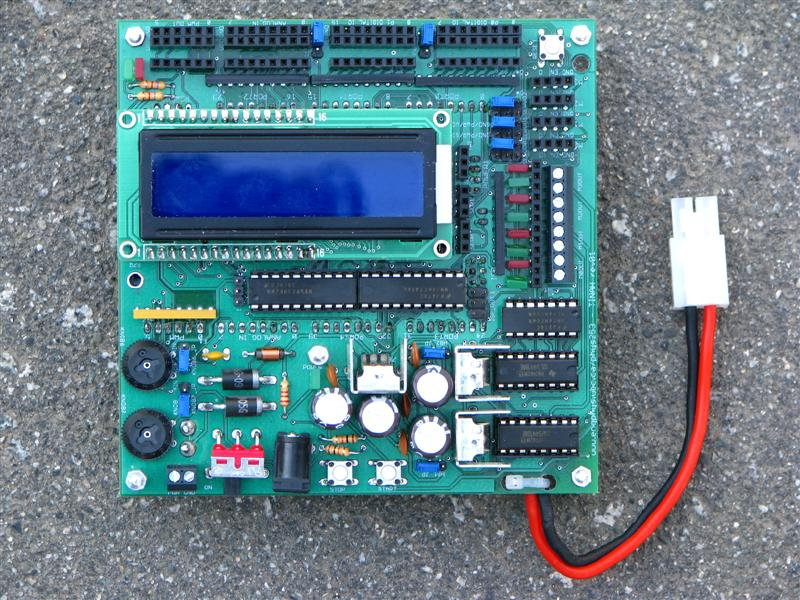
\includegraphics[scale=0.5]{TINAH.jpg}
          \vspace{7pt}
          \large{TINAH}
        \end{figure}
      \end{column}
    \end{columns}
  \end{frame} 
  

  \begin{frame}{What We Learned}
    \begin{itemize}
      \item <2->Design around available parts 
      \item <3->Solidworks before fabrication
      \item <4->Checklists \textgreater Time Dependent Goals
      \item <5->Organization
    \end{itemize}
  \end{frame} 
  

  \begin{frame}{References}
    \begin{itemize}
      \item \textbf{ENPH Logo:} \\http://ubc-rapid.com/blog/wp-content/uploads/2014/04/ENPHlogo.png
      \item \textbf{Challenge Surface:} \\http://projectlab.engphys.ubc.ca/wp-content/uploads/enph253-2014-CompetitionRules-v4.pdf
      \item \textbf{TINAH Picture:} \\http://projectlab.engphys.ubc.ca/enph253/tinah/
    \end{itemize}
  \end{frame}


\end{document}